% PREAMBLE
\documentclass[11pt]{amsart}
\usepackage[T1]{fontenc}
\usepackage{lmodern}
\usepackage{microtype}
\usepackage{amsmath,amssymb}
\usepackage{mathtools}
\usepackage{graphicx}
\usepackage{booktabs}
\usepackage{tikz}
\usepackage[colorlinks=true,linkcolor=blue!45!black,citecolor=blue!45!black,urlcolor=blue!45!black]{hyperref}
\usepackage[capitalize]{cleveref}

\newtheorem{theorem}{Theorem}[section]
\newtheorem{proposition}[theorem]{Proposition}
\newtheorem{lemma}[theorem]{Lemma}
\newtheorem{corollary}[theorem]{Corollary}
\newtheorem{conjecture}[theorem]{Conjecture}
\theoremstyle{definition}
\newtheorem{definition}[theorem]{Definition}
\newtheorem{fact}[theorem]{Fact}
\theoremstyle{remark}
\newtheorem{remark}[theorem]{Remark}

\title{Coprimality Density Above Dimension One}
\author{Carlo Mitchener}
\email{carlo.mitchener@gmail.com}
\date{2026-08-23}

% PAPER
\begin{document}

\begin{abstract}
Take a fractal built by keeping only certain digit patterns, and ask how often a point of it has coordinates with no common factor. This paper answers that for every such fractal of dimension greater than one. Fix a base $q \ge 2$, a dimension $D \ge 2$, and a set $F \subseteq \{0,\dots,q-1\}^D$ of admissible digit vectors, $k = |F|$; let $S_n$ be the $k^n$ points of $[0,q^n)^D$ whose base-$q$ digit vectors all lie in $F$, and let $A(n)$ count those with coordinate gcd $1$. If $F-F$ generates $\mathbb{Z}^D$ and $k > q$, then $A(n)/k^n \to B(F)\prod_{p \nmid q}(1-p^{-D})$, where $B(F) = \sum_{e \mid \mathrm{rad}(q)} \mu(e)k_e/k$ is an exact digit bracket. Away from the base the classical Euler factors survive untouched; at the base they are replaced, collectively and exactly, by $B(F)$, which at a composite base provably does not factor. The hypothesis $k>q$ says the attractor has dimension above one; on its own it is not enough. Consequences: the Sierpi\'nski gasket density $16/(3\pi^2)$; and, for $D$ even or $D=3$ with $B(F)>0$, that $A(n)$ satisfies no linear recurrence with constant rational coefficients.
\end{abstract}

\maketitle

\section{Introduction}
\label{sec:intro}

Stand at the origin of a square grid and look out. Some lattice points you can see; others hide exactly behind a nearer point on the same ray. A point $(x_1,x_2)$ is visible precisely when $\gcd(x_1,x_2)=1$, and the classical count says that $6/\pi^2$ of all lattice points are visible -- about $61\%$.

\begin{figure}[!ht]
\centering
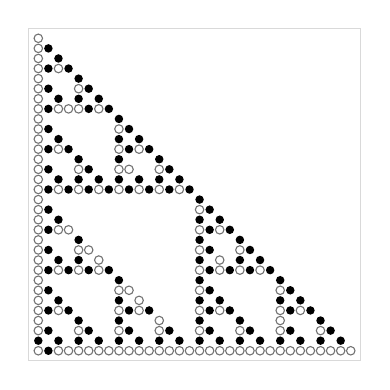
\begin{tikzpicture}[scale=0.128]
\draw[gray!30] (-1,-1) rectangle (32,32);
\foreach \x/\y in {1/0, 0/1, 2/1, 1/2, 4/1, 6/1, 5/2, 4/3, 1/4, 3/4, 2/5, 1/6, 8/1, 10/1, 9/2,
8/3, 12/1, 14/1, 13/2, 9/4, 8/5, 11/4, 8/7, 1/8, 3/8, 2/9, 1/10, 5/8, 4/9, 7/8, 4/11, 1/12,
2/13, 1/14, 16/1, 18/1, 17/2, 16/3, 20/1, 22/1, 21/2, 20/3, 17/4, 16/5, 19/4, 18/5, 17/6,
16/7, 24/1, 26/1, 25/2, 28/1, 30/1, 29/2, 28/3, 25/4, 24/5, 27/4, 26/5, 25/6, 24/7, 17/8,
16/9, 19/8, 17/10, 16/11, 21/8, 20/9, 23/8, 22/9, 21/10, 20/11, 17/12, 16/13, 19/12, 18/13,
17/14, 16/15, 1/16, 3/16, 2/17, 1/18, 5/16, 4/17, 7/16, 6/17, 5/18, 4/19, 1/20, 3/20, 2/21,
1/22, 9/16, 8/17, 11/16, 10/17, 8/19, 13/16, 12/17, 15/16, 14/17, 13/18, 12/19, 9/20, 8/21,
11/20, 10/21, 9/22, 8/23, 1/24, 2/25, 1/26, 5/24, 4/25, 7/24, 6/25, 5/26, 4/27, 1/28, 3/28,
2/29, 1/30}
  \fill[black] (\x,\y) circle (0.42);
\foreach \x/\y in {0/0, 2/0, 3/0, 0/2, 0/3, 4/0, 5/0, 6/0, 7/0, 4/2, 0/4, 0/5, 2/4, 0/6, 0/7,
8/0, 9/0, 10/0, 11/0, 8/2, 12/0, 13/0, 14/0, 15/0, 12/2, 12/3, 8/4, 10/4, 10/5, 8/6, 9/6,
0/8, 0/9, 2/8, 0/10, 0/11, 4/8, 6/8, 6/9, 4/10, 5/10, 0/12, 0/13, 2/12, 3/12, 0/14, 0/15,
16/0, 17/0, 18/0, 19/0, 16/2, 20/0, 21/0, 22/0, 23/0, 20/2, 16/4, 18/4, 16/6, 24/0, 25/0,
26/0, 27/0, 24/2, 24/3, 28/0, 29/0, 30/0, 31/0, 28/2, 24/4, 26/4, 24/6, 16/8, 18/8, 18/9,
16/10, 20/8, 22/8, 20/10, 16/12, 18/12, 16/14, 0/16, 0/17, 2/16, 0/18, 0/19, 4/16, 6/16,
4/18, 0/20, 0/21, 2/20, 0/22, 0/23, 8/16, 10/16, 8/18, 9/18, 12/16, 14/16, 12/18, 8/20,
10/20, 8/22, 0/24, 0/25, 2/24, 3/24, 0/26, 0/27, 4/24, 6/24, 4/26, 0/28, 0/29, 2/28, 0/30,
0/31}
  \draw[black!55] (\x,\y) circle (0.42);
\end{tikzpicture}
\caption{The level-$5$ Sierpi\'nski gasket design in $[0,32)^2$: the $243$ points whose binary digit pairs all avoid $(1,1)$. Filled dots are visible from the origin, $122$ of them; hollow dots hide behind a nearer point. The visible fraction tends to $16/(3\pi^2)$.}
\label{fig:gasket}
\end{figure}

Now look at a fractal instead of the whole grid. The Sierpi\'nski gasket can be built arithmetically: keep the points of $[0,2^n)^2$ whose binary digit pairs all avoid $(1,1)$. There are $3^n$ of them. \Cref{fig:gasket} shows the $243$ points at level $5$, filled where the point is visible from the origin and hollow where it is not.

The visible fraction on this fractal is not $6/\pi^2$. It is
\[
  \frac{16}{3\pi^2} \;=\; 0.540379646092\ldots,
\]
and the shape of that number is the whole story. Write it as
\[
  \underbrace{\tfrac{2}{3}}_{\text{the base}} \cdot \underbrace{\tfrac{6}{\pi^{2}}}_{1/\zeta(2)} \cdot \underbrace{\tfrac{4}{3}}_{(1-2^{-2})^{-1}} .
\]
The middle factor is the classical answer. The right factor cancels the classical Euler factor at the prime $2$, the base. The left factor is what the digit set puts back in its place: two of the three admissible digit pairs are not $(0,0)$, so exactly $\tfrac23$ of the points at every level have gcd odd. That last statement is an identity, exact at every finite level, with no error term at all.

This is the pattern in general, and it is the theorem of this paper. Every prime not dividing the base contributes its classical factor $1-p^{-D}$. Every prime dividing the base is deleted and the whole family of them is replaced, collectively, by one exact rational number $B(F)$ read off the digit set. At a prime base $B(F)$ is dull. At a composite base it is the entire content: the events ``the gcd is even'' and ``the gcd is divisible by $3$'' are correlated through the corner set, and $B(F)$ is provably not the product of its per-prime marginals (\cref{sec:factor}).

\medskip
\noindent\textbf{Where the hypothesis comes from.} The theorem needs the fractal to be more than one-dimensional. The attractor of the digit design has Hausdorff dimension $\alpha=\log_q k$, and the proof needs $\alpha>1$, i.e.\ $k>q$. The reason is one convergent series. Sieving out the primes dividing a gcd needs control on how many points of $S_n$ are divisible by a large modulus $m$; the sharp count is $O(k^n m^{-\alpha})$, and summing it against the von Mangoldt weight gives $-\zeta'(\alpha)/\zeta(\alpha)$, which converges exactly when $\alpha>1$. At $\alpha \le 1$ the series diverges and this route stops. That is not a blemish on the proof; it is where the mathematics genuinely changes.

The second hypothesis is that the differences $F-F$ generate all of $\mathbb{Z}^D$. Something like it is unavoidable: a design can be large and still arithmetically degenerate. Taking $q=3$, $D=2$ and $F=\{0,2\}^2$ gives $k=4>3$, dimension $\log_3 4 = 1.26$, and yet every coordinate of every point is even, so $A(n)=0$ forever while the formula predicts $0.512938\ldots$. So $k>q$ alone is insufficient (\cref{prop:sharp}). The consolation is pretty: shear that example by a factor of $2$ and the constant reappears untouched, one prime down.

\medskip
\noindent\textbf{What is new.} The method is standard: an elementary sieve driven by a regularity bound that is already known. The digit-box bound of \cref{lem:box} is the Ahlfors--David regularity of missing-digit sets, recorded as known in Chow, Varj\'u and Yu \cite{cvy}. What is new is the assembly: a $D$-dimensional statement about \emph{coupled} digits, where the coordinates of a point are chosen together and not independently; the exact bracket $B(F)$ at a composite base, together with a proof that it does not factor; and the resulting explicit constants. The literature we could find splits into two halves that do not meet. On one side, visible points of the \emph{full} lattice: Baake and Huck \cite{bh} study their dynamics as weak model sets, and Goins, Harris, Kubik and Mbirika \cite{ghkm} compute densities along generalized lines of sight. On the other side, one-dimensional arithmetic on digit-restricted integers: Banks and Shparlinski \cite{bs} study arithmetic functions such as $\varphi$ and $\sigma$ on such integers, and Erd\H{o}s, Mauduit and S\'ark\"ozy \cite{ems}, Konyagin \cite{kon} and Maynard \cite{may} prove distribution in residue classes uniformly over growing moduli. Nothing we found joins them. The uniformity of that last trio is exactly what a proof would need below dimension one; the route taken here deliberately avoids needing it, at the cost of the hypothesis $k>q$.

\medskip
\noindent\textbf{Guard.} The probability here is a lattice-arithmetic probability: pick a point uniformly from the finite set $S_n$, then let $n$ grow. It is not Lebesgue measure on the real attractor, where a point has no gcd at all. This is also what separates the result from \cite{bh}: there the ambient object is the full lattice $\mathbb{Z}^D$ with its natural density; here it is a sparse self-similar subset sampled level by level.

\section{Definitions}
\label{sec:defs}

\begin{definition}[design]
\label{def:design}
A \emph{design} is a triple $(q,D,F)$ with an integer base $q \ge 2$, a dimension $D \ge 2$, and a set $F \subseteq \{0,\dots,q-1\}^D$ of \emph{corners} with $k := |F| \ge 2$. Its level-$n$ set is
\[
  S_n \;=\; \Bigl\{\, \textstyle\sum_{j=0}^{n-1} q^{j} f_j \;:\; f_0,\dots,f_{n-1} \in F \,\Bigr\} \;\subseteq\; [0,q^{n})^{D},
\]
the sum taken coordinatewise. Base-$q$ expansion is injective on digit strings, so $|S_n| = k^n$. The \emph{census} of the design is
\[
  A(n) \;=\; \#\{\, x \in S_n \;:\; \gcd(x_1,\dots,x_D)=1 \,\},
\]
the number of points of $S_n$ visible from the origin.
\end{definition}

\begin{definition}[spanning, dimension, bracket]
\label{def:span}
Let $L = \langle F - F\rangle$ be the subgroup of $\mathbb{Z}^D$ generated by all differences of corners. The design is \emph{spanning} when $L = \mathbb{Z}^D$. Its \emph{dimension} is $\alpha = \log_q k$, the Hausdorff dimension of the attractor of the maps $x \mapsto (x+f)/q$, $f \in F$. For squarefree $e$ put
\[
  k_e \;=\; \#\{\, f \in F : e \mid f_i \text{ for every } i \,\},
  \qquad
  B(F) \;=\; \sum_{e \,\mid\, \mathrm{rad}(q)} \mu(e)\,\frac{k_e}{k},
\]
where $\mathrm{rad}(q)$ is the product of the distinct primes dividing $q$. We call $B(F)$ the \emph{bracket} of the design. It is a rational number in $[0,1]$.
\end{definition}

For a prime base $q=p$ the only digit vector divisible by $p$ is the zero vector, so $B(F) = 1 - \mathbf{1}[0 \in F]/k$. For composite $q$ the bracket sees the joint structure of the corner set, which is the point of \cref{sec:factor}.

\begin{definition}[predicted density]
\label{def:delta}
The \emph{predicted density} of a design is
\[
  \delta(q,D,F) \;=\; B(F) \prod_{p \,\nmid\, q}\bigl(1-p^{-D}\bigr)
  \;=\; \frac{B(F)}{\zeta(D)} \prod_{p \,\mid\, q}\bigl(1-p^{-D}\bigr)^{-1}.
\]
\end{definition}

Throughout, $e(x) = \exp(2\pi i x)$, $\Lambda$ is the von Mangoldt function, $\mathrm{ord}_d(q)$ is the multiplicative order of $q$ modulo $d$, and $\|y\|$ is the distance from $y$ to the nearest integer. We write
\[
  T_m(n) = \#\{x \in S_n : m \mid x_i \ \forall i\},
  \qquad
  T^{*}_m(n) = \#\{x \in S_n \setminus \{0\} : m \mid x_i \ \forall i\}.
\]
The starred version matters: if $0 \in F$ then $0 \in S_n$ and every modulus divides it, so unstarred tails over all $m$ diverge for a trivial reason.

\section{Results}
\label{sec:results}

\subsection{The theorem}

\begin{theorem}[coprimality density above dimension one]
\label{thm:main}
Let $(q,D,F)$ be a design with $D \ge 2$ that is spanning and satisfies $k > q$, equivalently $\alpha = \log_q k > 1$. Then
\[
  \lim_{n \to \infty} \frac{A(n)}{k^{n}}
  \;=\; \delta \;=\; B(F)\prod_{p \,\nmid\, q}\bigl(1-p^{-D}\bigr)
  \;=\; \frac{B(F)}{\zeta(D)}\prod_{p \,\mid\, q}\bigl(1-p^{-D}\bigr)^{-1}.
\]
The value $B(F)=0$ is permitted and then $\delta = 0$; this happens exactly when every corner of $F$ has all coordinates divisible by some prime dividing $q$, and in particular whenever $F$ is contained in the corners divisible by a fixed prime $p \mid q$.
\end{theorem}

The proof occupies \cref{sec:proofs}. It has three moving parts: an exact identity at the base (\cref{prop:base}), a uniform character contraction driven by the spanning hypothesis (\cref{lem:contract}), and a digit-box bound whose Chebyshev sum converges precisely when $\alpha>1$ (\cref{lem:box,lem:cheb}).

\begin{proposition}[the base is exact at every finite level]
\label{prop:base}
For every design, every squarefree $e \mid \mathrm{rad}(q)$ and every $n \ge 1$,
\[
  T_e(n) \;=\; k_e\,k^{\,n-1},
  \qquad\text{and}\qquad
  \#\{x \in S_n : \gcd(\gcd(x), q) = 1\} = B(F)k^{n}.
\]
Neither spanning nor $k>q$ is needed. If $q=p$ is prime, then for every $a$ with $1 \le a \le n$,
$\#\{x \in S_n : p^{a} \mid \gcd(x)\} = \mathbf{1}[0 \in F]^{a}\,k^{\,n-a}$.
\end{proposition}

\begin{corollary}[the gasket]
\label{cor:gasket}
For $q=2$, $D=2$, $F = \{(0,0),(1,0),(0,1)\}$ -- the Sierpi\'nski gasket design, $k=3$, spanning, $\alpha = \log_2 3 = 1.585 > 1$ -- the census satisfies
\[
  \frac{A(n)}{3^{n}} \;\longrightarrow\; \frac{2}{3}\cdot\frac{6}{\pi^{2}}\cdot\frac{4}{3}
  \;=\; \frac{16}{3\pi^{2}} \;=\; 0.540379646092\ldots
\]
The integer sequence $A(n)$ is \href{https://oeis.org/A396934}{OEIS A396934}, whose terms for $n \ge 1$ begin
\[
  2,\; 4,\; 12,\; 34,\; 122,\; 362,\; 1130,\; 3406,\; 10506,\; 31550,\; 95260
\]
(the entry has offset $0$ and records $a(0)=0$, matching $A(0)=0$). That entry carries the conjecture that $a(n)/3^{n}$ converges to $16/(3\pi^{2})$; \cref{thm:main} settles it.
\end{corollary}

\begin{proof}
The design is spanning because $(1,0)-(0,0)$ and $(0,1)-(0,0)$ are the standard basis, and $k = 3 > 2 = q$. Only $(0,0)$ has both coordinates even, so $k_2 = 1$ and $B(F) = 1 - 1/3 = 2/3$ by \cref{def:span}. \Cref{thm:main} gives $\delta = (2/3)\zeta(2)^{-1}(1-2^{-2})^{-1} = (2/3)(6/\pi^{2})(4/3)$.
\end{proof}

The same one-line computation settles a family of named designs at once. \Cref{tab:constants} lists them with their digit sets written out in full; each is spanning with $k>q$, so \cref{thm:main} applies to every row.

\begin{table}[ht]
\centering
\small
\begin{tabular}{llll}
\toprule
design & $(q,D)$, $k$ & $B(F)$ & $\delta$ \\
\midrule
gasket & $(2,2)$, $3$ & $2/3$ & $16/(3\pi^{2}) = 0.540379646092$ \\
or-triangle & $(2,2)$, $3$ & $1$ & $8/\pi^{2} = 0.810569469139$ \\
carpet & $(3,2)$, $8$ & $7/8$ & $189/(32\pi^{2}) = 0.598428240888$ \\
Vicsek plus & $(3,2)$, $5$ & $1$ & $27/(4\pi^{2}) = 0.683917989586$ \\
Menger sponge & $(3,3)$, $20$ & $19/20$ & $(513/520)/\zeta(3) = 0.820708619488$ \\
\bottomrule
\end{tabular}
\caption{Named designs closed by \cref{thm:main}. Digit sets: the gasket is $\{(0,0),(1,0),(0,1)\}$, the or-triangle $\{(1,0),(0,1),(1,1)\}$, the carpet $\{0,1,2\}^{2}\setminus\{(1,1)\}$, the Vicsek plus $\{(1,0),(0,1),(1,1),(2,1),(1,2)\}$. The carpet omits the centre corner; the Vicsek plus is the five corners with at least one coordinate equal to $1$ and, in $\{0,2\}^2$, none; the Menger sponge is the $20$ corners of $\{0,1,2\}^{3}$ with at most one coordinate equal to $1$. The Vicsek plus has $0 \notin F$, so no point of it ever has gcd divisible by $3$, and its density therefore exceeds the classical $6/\pi^{2}$.}
\label{tab:constants}
\end{table}

\subsection{Sharpness, and a shear that repairs it}

\begin{proposition}[$k>q$ alone is insufficient]
\label{prop:sharp}
Let $q=3$, $D=2$, $F = \{0,2\}^{2}$, the Cantor dust design. Then $k = 4 > 3 = q$ and $\alpha = \log_3 4 = 1.2619 > 1$, but $A(n) = 0$ for every $n \ge 1$, while $\delta(3,2,F) = 81/(16\pi^{2}) = 0.512938\ldots > 0$. Hence the conclusion of \cref{thm:main} fails without a hypothesis on $\langle F-F\rangle$.
\end{proposition}

\begin{proof}
Every corner has both coordinates even and $q=3$ is odd, so by induction on $n$ every coordinate of every point of $S_n$ is even and $\gcd(x) \ge 2$; thus $A(n)=0$. Here $\langle F-F\rangle = 2\mathbb{Z}^{2}$ has index $4$, and $2 \nmid q$, so the design is not spanning and condition (E) fails as well. For the predicted value: $\mathrm{rad}(3)=3$, and the only corner with both coordinates divisible by $3$ is $(0,0)$, so $k_3 = 1$ and $B(F) = 1 - 1/4 = 3/4$; hence
\[
  \delta \;=\; \tfrac34 \cdot \zeta(2)^{-1} \cdot (1-3^{-2})^{-1}
  \;=\; \tfrac34\cdot\tfrac{6}{\pi^{2}}\cdot\tfrac98 \;=\; \frac{81}{16\pi^{2}} \;=\; 0.512938\ldots,
\]
which is positive while the truth is zero.
\end{proof}

This says $k>q$ alone is insufficient. It does \emph{not} say spanning is necessary: designs of index $>1$ whose index has all its prime factors dividing $q$ appear to obey the formula unchanged, which is \cref{con:E} below. And the counterexample is not a dead end.

\begin{proposition}[the shear repair]
\label{prop:shear}
With $q=3$, $D=2$, $F = \{0,2\}^{2}$ as in \cref{prop:sharp}, let $G = \{0,1\}^{2}$ at the same base. Then $x \mapsto 2x$ is a bijection $S_n(G) \to S_n(F)$ carrying $\gcd(y)$ to $2\gcd(y)$, the design $G$ is spanning with $k=4>3$, and consequently
\[
  \frac{\#\{x \in S_n(F) : \gcd(x) = 2\}}{4^{n}}
  \;\longrightarrow\; \frac{3}{4}\cdot\frac{6}{\pi^{2}}\cdot\frac{9}{8}
  \;=\; \frac{81}{16\pi^{2}} \;=\; 0.512938\ldots
\]
\end{proposition}

\begin{proof}
Digitwise, multiplication by $2$ sends the digit vector $g \in \{0,1\}^2$ to $2g \in \{0,2\}^2$ with no carries, since $2 \cdot 1 = 2 < 3$; so it maps $S_n(G)$ bijectively onto $S_n(F)$ and multiplies every coordinate by $2$, hence multiplies the gcd by $2$. Thus $\gcd(x)=2$ for $x = 2y$ exactly when $\gcd(y)=1$. The design $G$ contains $(0,0),(1,0),(0,1)$, so its differences contain the standard basis and it is spanning; $k = 4 > 3$; only $(0,0)$ has both coordinates divisible by $3$, so $k_3 = 1$ and $B(G) = 3/4$. Apply \cref{thm:main} to $G$.
\end{proof}

So the constant survives the failure, one prime down: the dust is not outside the theory, it is the theory read on the sublattice $2\mathbb{Z}^2$.

\subsection{The composite base does not factor}
\label{sec:factor}

At a prime base the bracket is $1 - \mathbf{1}[0\in F]/k$ and carries no information beyond whether the origin corner is filled. At a composite base it carries all of it, because divisibility of the gcd by the different primes dividing $q$ is correlated through the corner set. The cleanest witness is a base-$6$ design.

\begin{fact}[non-factorization at a composite base]
\label{fact:factor}
Let $q=6$, $D=2$ and
\[
  F \;=\; \{(0,0),(0,3),(1,1),(1,2),(2,0),(2,1),(4,0),(5,5)\},
  \qquad k = 8 .
\]
Then $k_2 = 3$, $k_3 = 2$, $k_6 = 1$, so
\[
  B(F) \;=\; 1 - \tfrac38 - \tfrac28 + \tfrac18 \;=\; \tfrac12,
  \qquad\text{whereas}\qquad
  \Bigl(1-\tfrac38\Bigr)\Bigl(1-\tfrac28\Bigr) \;=\; 0.46875 .
\]
The number of points of $S_n$ whose gcd is coprime to $6$ is exactly $k^{n}/2$ at every level, verified on the integer for $1 \le n \le 6$:
\begin{center}
\begin{tabular}{rrrr}
\toprule
$n$ & $|S_n| = 8^{n}$ & gcd coprime to $6$ & naive $0.46875 \cdot 8^{n}$ \\
\midrule
$3$ & $512$ & $256$ & $240$ \\
$4$ & $4096$ & $2048$ & $1920$ \\
$5$ & $32768$ & $16384$ & $15360$ \\
$6$ & $262144$ & $131072$ & $122880$ \\
\bottomrule
\end{tabular}
\end{center}
Checked by \texttt{scripts/verify.py}.
\end{fact}

The identity $B(F)k^n$ is \cref{prop:base} with inclusion-exclusion over $\{2,3\}$, so the left column is Proved; the table is the finite domain on which it was re-run to the integer. The design is spanning with $k=8>6$, so \cref{thm:main} applies and its density is
\[
  \delta \;=\; \tfrac12 \cdot \tfrac{6}{\pi^{2}} \cdot \tfrac{4}{3} \cdot \tfrac{9}{8}
  \;=\; \frac{9}{2\pi^{2}} \;=\; 0.455945326391\ldots
\]
A single base can carry two different brackets at the same $k$: the base-$6$ design $\{(0,0),(0,1),(1,0),(1,1),(2,3),(3,2),(4,5),(5,4)\}$ also has $k=8$ but $B=7/8$ and $\delta = 0.797904321183\ldots$. The same contrast occurs at base $4$ with $B \in \{3/4, 7/8\}$ at $k=8$. No product of per-prime marginals reproduces both.

\subsection{Exact enumeration}

\begin{fact}[ten spanning designs, exhaustively enumerated]
\label{fact:census}
For each of the ten spanning designs of \cref{tab:endpoints}, every point of $S_n$ was enumerated -- no sampling, no subsampling -- for every level $n$ from $1$ to the stated $N$, the coordinate gcd computed by the Euclidean algorithm, and $A(n)$ counted exactly. In every one of those $67$ level rows the identity $\#\{x \in S_n : \gcd(\gcd(x),q)=1\} = B(F)k^{n}$ of \cref{prop:base} held on the integer. Each of the ten designs was confirmed spanning, its lattice index $[\mathbb{Z}^{D}:\langle F-F\rangle]$ coming out $1$ by exact integer row reduction; and for each of the ten, as for the five designs of \cref{tab:constants}, the value of $\delta$ was recomputed from \cref{def:span,def:delta} by exact rational arithmetic on the digit set and agreed to $10^{-12}$ with the closed form recorded in \cref{sec:repro}. The domain is exactly: gasket and or-triangle $1 \le n \le 11$; carpet, $q=4$ pair and $q=6$ first design $1 \le n \le 5$; Vicsek plus $1 \le n \le 7$; $q=5$ pair $1 \le n \le 6$; $q=6$ second design $1 \le n \le 6$. Checked by \texttt{scripts/verify.py}.
\end{fact}

\begin{table}[ht]
\centering
\small
\begin{tabular}{lrrrlrr}
\toprule
design & $q$ & $D$ & $k$ & $B(F)$ & $\delta$ & $A(N)/k^{N}-\delta$ \\
\midrule
or-triangle & $2$ & $2$ & $3$ & $1$   & $0.810569469139$ & $+0.001231$ \\
gasket      & $2$ & $2$ & $3$ & $2/3$ & $0.540379646092$ & $-0.002634$ \\
carpet      & $3$ & $2$ & $8$ & $7/8$ & $0.598428240888$ & $-0.013162$ \\
Vicsek plus & $3$ & $2$ & $5$ & $1$   & $0.683917989586$ & $+0.008818$ \\
$q=4$ rows  & $4$ & $2$ & $8$ & $3/4$ & $0.607927101854$ & $-0.025041$ \\
$q=4$ border& $4$ & $2$ & $8$ & $7/8$ & $0.709248285496$ & $-0.017262$ \\
$q=5$ binary& $5$ & $3$ & $7$ & $1$   & $0.838616303005$ & $+0.022810$ \\
$q=5$ axes  & $5$ & $3$ & $7$ & $6/7$ & $0.718813974004$ & $-0.043713$ \\
$q=6$ first & $6$ & $2$ & $8$ & $7/8$ & $0.797904321183$ & $-0.008079$ \\
$q=6$ second& $6$ & $2$ & $8$ & $1/2$ & $0.455945326391$ & $-0.004361$ \\
\bottomrule
\end{tabular}
\caption{Endpoint of the enumerated domain of \cref{fact:census}, with the \emph{signed} error at the top level $N$. Digit sets, in the same order: $\{(1,0),(0,1),(1,1)\}$; $\{(0,0),(1,0),(0,1)\}$; $\{0,1,2\}^2 \setminus \{(1,1)\}$; $\{(1,0),(0,1),(1,1),(2,1),(1,2)\}$; $\{0,1\}\times\{0,1,2,3\}$; $\{(0,0),(0,1),(0,3),(1,0),(1,3),(3,0),(3,2),(3,3)\}$; $\{0,1\}^3\setminus\{(0,0,0)\}$; $\{(0,0,0)\} \cup \{c\,e_i : c \in \{1,2\},\, 1 \le i \le 3\}$; $\{(0,0),(0,1),(1,0),(1,1),(2,3),(3,2),(4,5),(5,4)\}$; $\{(0,0),(0,3),(1,1),(1,2),(2,0),(2,1),(4,0),(5,5)\}$.}
\label{tab:endpoints}
\end{table}

\begin{remark}[rate honesty]
\label{rem:rate}
\Cref{tab:endpoints} is evidence of convergence and nothing more. The proof supplies no useful rate: chaining \cref{lem:box,lem:cheb} with the sieve of \cref{sec:proofs} gives an error only of order $(\log n)^{1-\alpha}$, which is qualitative, while the measured errors are far smaller. Nor is the numerical behaviour monotone. The signed errors of the last four levels of the or-triangle run $-0.021970$, $-0.000530$, $-0.002021$, $+0.001231$, and of the Vicsek plus $-0.015118$, $+0.013042$, $-0.008078$, $+0.008818$: they change sign, so no rate can be read off them. Convergence is also slow for some designs: the $q=5$, $D=3$ axes design is still $4.4 \times 10^{-2}$ from $\delta$ at the top of the enumerated domain. The table must not be read as confirming a geometric rate; it confirms only the values it lists.
\end{remark}

\subsection{No linear recurrence}

\begin{theorem}[the C-finite obstruction]
\label{thm:cfinite}
Let $A(n)$ be a sequence of integers and $k \ge 2$ an integer with $A(n)/k^{n} \to \delta$ and $\delta$ irrational. Then $A$ satisfies no linear recurrence with constant rational coefficients, of any order.
\end{theorem}

\begin{corollary}[census sequences are not C-finite]
\label{cor:cfinite}
Let $(q,D,F)$ be spanning with $D \ge 2$, $k>q$ and $B(F) > 0$. If $D$ is even, or $D = 3$, then the census $A(n)$ satisfies no linear recurrence with constant rational coefficients. In particular \href{https://oeis.org/A396934}{A396934} is not C-finite.
\end{corollary}

\begin{proof}
By \cref{thm:main}, $A(n)/k^n \to \delta = B(F)\zeta(D)^{-1}\prod_{p \mid q}(1-p^{-D})^{-1}$. Every factor other than $\zeta(D)^{-1}$ is a rational number, and their product is nonzero because $B(F)>0$. For even $D$, Euler's evaluation makes $\zeta(D)$ a nonzero rational multiple of $\pi^{D}$, so $\delta$ is a nonzero rational multiple of $\pi^{-D}$, irrational by the transcendence of $\pi$ \cite{lindemann}. For $D=3$, $\zeta(3)$ is irrational by Ap\'ery \cite{apery}, hence so is any nonzero rational multiple of $\zeta(3)^{-1}$. Apply \cref{thm:cfinite}.
\end{proof}

The hypothesis $B(F)>0$ is not decoration. If $B(F)=0$ then $\delta = 0$, which is rational, and the argument says nothing; indeed a design with $A(n)=0$ for all $n$ satisfies every recurrence. Four doors stay open, and we state them as open rather than dress them up: odd $D \ge 5$, where the irrationality of $\zeta(D)$ is not known; $B(F)=0$; $k \le q$, where \cref{thm:main} itself is unproved; and recurrences with polynomial coefficients, i.e.\ $P$-recursive or holonomic sequences, which exhaustive exact fitting with held-out terms has failed to find but which no argument here excludes.

\subsection{An exhaustive census in dimension four}

Where does \cref{thm:main} bite? In the smallest interesting case one can simply look at every design at once. Take $q=2$, $D=4$: a design is any subset of the $16$ vertices of the $4$-cube, so there are $2^{16} = 65536$ of them. The hyperoctahedral group $B_4$ of signed coordinate permutations has order $2^4 \cdot 4! = 384$ and acts on these subsets.

\begin{fact}[the base-$2$, $D=4$ census]
\label{fact:d4}
Under the action of the order-$384$ group $B_4$, the $65536$ subsets of the $4$-cube fall into exactly $402$ orbits. Taking the minimum bitmask in each orbit as its representative: $400$ representatives have $k \ge 2$, $396$ have $k > 2$, and $336$ are both spanning and $k>2$, hence satisfy the hypotheses of \cref{thm:main}; the remaining $66$ orbits do not. Among the $400$ eligible representatives the quadruples $(A(1),A(2),A(3),A(4))$ take $189$ distinct values, with $87$ values attained more than once. Checked by \texttt{scripts/verify.py}, which recomputes all of it by a second implementation independent of the one that produced it: orbits by union--find over four group generators rather than by applying all $384$ elements, and the lattice index by integer row reduction rather than by the gcd of all $4\times4$ minors. The orbit counts for $D = 0,1,2,3,4$ are $2, 3, 6, 22, 402$; these are $A000616(D)$ for $0 \le D \le 4$, the entry \href{https://oeis.org/A000616}{OEIS A000616} having offset $-1$ and its data beginning with a conventional $a(-1)=1$. The identification is the one that entry records itself: $A000616(D)$ counts the inequivalent binary codes of length $D$, that is, the subsets of $\{0,1\}^{D}$ up to $B_D$.
\end{fact}

\begin{remark}[what the group does and does not preserve]
\label{rem:orbit}
$B_4$ contains coordinate complementations $v_i \mapsto 1-v_i$, which move the arithmetic origin. They therefore do \emph{not} preserve $B(F)$, $\delta$ or $A(n)$; only $k$ and the property of being spanning are orbit invariants. Every count in \cref{fact:d4} that involves $B(F)$ or $A(n)$ -- that is, the $189$ and the $87$ -- is a statement about the explicit minimum-bitmask representative of each orbit and not an intrinsic statement about the orbit. Some minimum representatives contain the corner $0$ and some do not, giving brackets $1-1/k$ and $1$ respectively. For every one of these designs $\delta = B(F)\cdot 96/\pi^{4}$, since $\zeta(4)^{-1}(1-2^{-4})^{-1} = (90/\pi^{4})(16/15)$. Finally, equality of four initial terms is not equality of sequences; the $87$ collisions are a finite-level observation.
\end{remark}

\subsection{A conjecture, with its failure mode}

\begin{conjecture}[the wider hypothesis]
\label{con:E}
\Cref{thm:main} holds with ``spanning'' replaced by condition (E): $F-F$ has full rank $D$, and every prime dividing the index $[\mathbb{Z}^{D} : \langle F-F\rangle]$ divides $q$. Evidence: every design of index $>1$ satisfying (E) that we enumerated obeys the formula unchanged, including designs of index $4$ constructed at bases $4$ and $6$; and the base peel of \cref{lem:peel} formally survives an index whose primes all divide $q$, since such an index is invisible to every modulus coprime to $q$. Failure mode: (E) is not cosmetic, and beyond it the conclusion is false in a strong sense. For $q=7$, $D=2$, $F = \{v \in \{0,\dots,6\}^{2} : v_1+v_2 \equiv 1 \bmod 3\}$ one has $k=16>7$ and index $3$, with $3 \nmid 7$; the ratio $A(n)/k^{n}$ does not converge at all but has three period-$3$ subsequential limits, near $0.698175$, $0.698175$ and $0.465450$. So a proof of the conjecture must use the divisibility in (E) and not merely full rank; and the honest reading of \cref{prop:sharp} together with this example is that the arithmetic of the index, not the dimension, is what governs the boundary.
\end{conjecture}

\section{Proofs}
\label{sec:proofs}

Throughout this section $(q,D,F)$ is a design, $k=|F|$, and $\alpha = \log_q k$.

\subsection{The base}

\begin{proof}[Proof of \cref{prop:base}]
Let $e \mid \mathrm{rad}(q)$ be squarefree. Every prime dividing $e$ divides $q$ and $e$ is squarefree, so $e \mid q$. Write a point of $S_n$ as $x = f_0 + q y$ with $f_0 \in F$ the least significant digit vector and $y \in S_{n-1}$; the map $(f_0,y) \mapsto x$ is a bijection $F \times S_{n-1} \to S_n$. Since $e \mid q$ we have $e \mid q y_i$ for every $i$, so $e \mid x_i$ for all $i$ if and only if $e \mid (f_0)_i$ for all $i$. The last digit vector is thus pinned to one of the $k_e$ corners counted by $k_e$ and the remaining $n-1$ digit vectors are free, giving $T_e(n) = k_e k^{n-1}$ exactly, at every level, with no error term.

For the second statement, $\gcd(\gcd(x),q)=1$ says that no prime dividing $q$ divides all of $x_1,\dots,x_D$. By inclusion--exclusion over the distinct primes dividing $q$, the count is $\sum_{e \mid \mathrm{rad}(q)} \mu(e) T_e(n) = k^{n-1}\sum_e \mu(e)k_e = B(F)k^n$.

For prime $q=p$: the only $f \in \{0,\dots,p-1\}^{D}$ with $p \mid f_i$ for all $i$ is $f = 0$. Hence $p \mid \gcd(x)$ forces $f_0 = 0$, which requires $0 \in F$, and then $x = py$ with $y \in S_{n-1}$ and $\gcd(x) = p\gcd(y)$. Iterating this $a$ times, which needs $a \le n$, gives the stated formula. The restriction $a \le n$ is not cosmetic: if $0 \in F$ and $a > n$ the left side is $1$, counting the origin alone, while $k^{\,n-a}$ is not even an integer.
\end{proof}

\subsection{Away from the base}

\begin{lemma}[character contraction]
\label{lem:contract}
Let the design be spanning. Let $d \ge 2$ with $\gcd(d,q)=1$, let $t \in (\mathbb{Z}/d)^{D}$ be nonzero, and set $r = \mathrm{ord}_d(q)$ and
\[
  f_l(t) \;=\; \frac{1}{k}\Bigl| \sum_{v \in F} e\bigl(q^{l}\langle t, v\rangle / d\bigr) \Bigr| .
\]
Then
\[
  \prod_{l=0}^{r-1} f_l(t) \;\le\; c(q,k) \;:=\; 1 - \frac{2}{k}\Bigl(1 - \cos\frac{\pi}{2q}\Bigr) \;<\; 1 .
\]
The constant depends only on $q$ and $k$, not on $d$, $t$, or which corners $F$ holds.
\end{lemma}

\begin{proof}
First, spanning produces a useful difference. If $\langle t, v-v'\rangle \equiv 0 \bmod d$ for all $v,v' \in F$, then $t$ annihilates $F-F$, hence annihilates the group $\langle F-F\rangle = \mathbb{Z}^D$ it generates, hence $t \equiv 0$, contrary to assumption. So fix $v,v' \in F$ with
\[
  \Delta := \langle t, v - v'\rangle \not\equiv 0 \pmod d .
\]

Second, the orbit of $\Delta/d$ under multiplication by $q$ cannot stay near an integer. Put $y_l = \|q^{l}\Delta/d\|$. Since $\gcd(q,d)=1$, multiplication by $q$ permutes $\mathbb{Z}/d$, so the sequence $q^{l}\Delta \bmod d$ is purely periodic with period $r' \mid r$ and never $\equiv 0$; hence $y_l \ge 1/d > 0$ for all $l$. Suppose, for contradiction, that $y_l < 1/(2q)$ for every $l$ in one full period $0 \le l < r'$. If $y_l < 1/(2q)$ then $q^{l}\Delta/d$ is within $1/(2q)$ of an integer $N$, so $q^{l+1}\Delta/d$ is within $1/2$ of the integer $qN$, and therefore $y_{l+1} = q\,y_l$ exactly. Applying this $r'$ times around the period returns to the start: $y_0 = y_{r'} = q^{r'} y_0$. As $y_0 > 0$ and $q^{r'} > 1$, this is impossible. So there is some $l_0$ in the period with $y_{l_0} \ge 1/(2q)$; and of course $y_{l_0} \le 1/2$ by definition of $\|\cdot\|$.

Third, one large $y_l$ contracts the sum. At $l = l_0$ split the character sum into the two terms coming from $v,v'$ and the other $k-2$ terms. For unit complex numbers, $|e(a)+e(b)| = 2|\cos(\pi(a-b))|$, and here $a - b = q^{l_0}\langle t, v-v'\rangle/d = q^{l_0}\Delta/d$, whose distance to the nearest integer is $y_{l_0} \in [1/(2q), 1/2]$. Since $\cos$ is even, $2\pi$-periodic and decreasing on $[0,\pi/2]$, we get $|\cos(\pi(a-b))| = \cos(\pi y_{l_0}) \le \cos(\pi/(2q))$. Bounding the other terms by $1$ each,
\[
  \Bigl|\sum_{v \in F} e\bigl(q^{l_0}\langle t,v\rangle/d\bigr)\Bigr|
  \;\le\; (k-2) + 2\cos\frac{\pi}{2q},
\]
so $f_{l_0}(t) \le 1 - \frac{2}{k}\bigl(1-\cos\frac{\pi}{2q}\bigr) = c(q,k)$. Every other factor $f_l(t)$ is at most $1$ by the triangle inequality, and $r' \mid r$ so the period sits inside the product. The claim follows, and $c(q,k)<1$ because $\cos(\pi/(2q))<1$ for $q \ge 2$.
\end{proof}

\begin{corollary}[equidistribution rate]
\label{cor:equi}
Let the design be spanning, $\gcd(d,q)=1$, and $a \in (\mathbb{Z}/d)^{D}$. Then
\[
  \Bigl| \frac{\#\{x \in S_n : x \equiv a \bmod d\}}{k^{n}} - \frac{1}{d^{D}} \Bigr|
  \;\le\; c(q,k)^{\lfloor n/\mathrm{ord}_d(q)\rfloor}.
\]
\end{corollary}

\begin{proof}
A point $x \in S_n$ is $\sum_{l<n} q^{l} f_l$, so for $t \in (\mathbb{Z}/d)^{D}$,
\[
  \sum_{x \in S_n} e\bigl(\langle t, x\rangle/d\bigr) \;=\; \prod_{l=0}^{n-1} \sum_{v \in F} e\bigl(q^{l}\langle t, v\rangle/d\bigr),
\]
the digits being chosen independently. By orthogonality of additive characters on $(\mathbb{Z}/d)^{D}$,
\[
  \#\{x \in S_n : x \equiv a\} \;=\; \frac{1}{d^{D}} \sum_{t} e\bigl(-\langle t,a\rangle/d\bigr) \prod_{l<n} \sum_{v\in F} e\bigl(q^{l}\langle t,v\rangle/d\bigr).
\]
The term $t=0$ contributes $k^{n}/d^{D}$. For each nonzero $t$ the modulus of its term is $k^{n}\prod_{l<n} f_l(t)$, and the $n$ factors contain $\lfloor n/r \rfloor$ complete periods of the orbit $l \mapsto q^{l}t$, each contributing at most $c(q,k)$ by \cref{lem:contract}, the remaining factors being at most $1$. There are $d^{D}-1 < d^{D}$ nonzero $t$, and dividing by $d^{D}$ absorbs that count. The bound follows.
\end{proof}

\begin{corollary}[base peel]
\label{lem:peel}
Let the design be spanning and let $d = em$ be squarefree with $e \mid \mathrm{rad}(q)$ and $\gcd(m,q)=1$. Then
\[
  \frac{T_d(n)}{k^{n}} \;=\; \frac{k_e}{k}\cdot\frac{1}{m^{D}} \;+\; O\bigl(c(q,k)^{\lfloor (n-1)/\mathrm{ord}_m(q)\rfloor}\bigr),
\]
with an absolute implied constant. In particular, at fixed $d$, $T_d(n)/k^{n} \to (k_e/k)m^{-D}$ as $n \to \infty$.
\end{corollary}

\begin{proof}
Write $x = f_0 + qy$ with $f_0 \in F$, $y \in S_{n-1}$. By the argument of \cref{prop:base}, $e \mid x_i$ for all $i$ if and only if $e \mid (f_0)_i$ for all $i$, a condition on $f_0$ alone, met by exactly $k_e$ corners. The condition $m \mid x_i$ for all $i$ reads $qy \equiv -f_0 \bmod m$, and $q$ is invertible mod $m$, so it is the single congruence $y \equiv -q^{-1}f_0 \bmod m$, a condition on $y$ alone. The two conditions are therefore independent given $f_0$, and
\[
  T_d(n) \;=\; \sum_{\substack{f_0 \in F \\ e \mid (f_0)_i\ \forall i}} \#\{y \in S_{n-1} : y \equiv -q^{-1}f_0 \bmod m\}.
\]
By \cref{cor:equi} each inner count is $k^{n-1}(m^{-D} + O(c^{\lfloor (n-1)/\mathrm{ord}_m q\rfloor}))$, and there are $k_e$ terms. Divide by $k^{n}$.
\end{proof}

\subsection{The digit box, and why dimension one is the barrier}

\begin{lemma}[digit-box bound]
\label{lem:box}
For every design, every $m \ge 2$ and every $0 \le h \le n$,
\[
  T_m(n) \;\le\; k^{\,n-h}\Bigl(\frac{q^{h}}{m}+1\Bigr)^{D}.
\]
Consequently, for the count over nonzero points,
\[
  T^{*}_m(n) \;\le\; (q+1)^{D}\,k^{n}\,m^{-\alpha} \text{ for all } m \ge 2,
  \qquad T^{*}_m(n) = 0 \text{ for } m \ge q^{n}.
\]
\end{lemma}

\begin{proof}
Split the digit string at position $h$: every $x \in S_n$ is uniquely $x = x_{\mathrm{lo}} + q^{h}x_{\mathrm{hi}}$ with $x_{\mathrm{lo}} \in S_h$ and $x_{\mathrm{hi}} \in S_{n-h}$, because base-$q$ digits do not interact. There are $k^{n-h}$ choices of $x_{\mathrm{hi}}$. Fix one. The condition $m \mid x_i$ pins each coordinate $(x_{\mathrm{lo}})_i$ to a single residue class modulo $m$, and $S_h \subseteq [0,q^{h})^{D}$, so each coordinate has at most $\lfloor q^{h}/m\rfloor + 1 \le q^{h}/m + 1$ admissible values in $[0,q^{h})$. Bounding $x_{\mathrm{lo}}$ by the full box gives at most $(q^{h}/m+1)^{D}$ choices, whence the first display.

Now take $m$ with $2 \le m < q^{n}$ and choose $h = \lceil \log_q m\rceil$, so that $1 \le h \le n$ and $m \le q^{h} < qm$. Then $q^{h}/m + 1 < q + 1$, and $k^{h} = q^{h\alpha} \ge m^{\alpha}$, so $k^{n-h} = k^{n}/k^{h} \le k^{n}m^{-\alpha}$. Substituting gives $T_m(n) \le (q+1)^{D}k^{n}m^{-\alpha}$, and $T^{*}_m(n) \le T_m(n)$. For $m \ge q^{n}$, a nonzero $x \in S_n$ has some coordinate in $(0,q^{n}) \subseteq (0,m)$, which cannot be divisible by $m$; so $T^{*}_m(n) = 0$, and the displayed bound holds trivially there.
\end{proof}

This bound is not new. It is the Ahlfors--David regularity of missing-digit sets, recorded as known in Chow, Varj\'u and Yu \cite[\S1]{cvy}; what is new here is only its use, to close a $D$-dimensional coprimality sieve on a set whose coordinates are coupled through $F$.

\begin{lemma}[Chebyshev sum]
\label{lem:cheb}
Suppose $\alpha > 1$, i.e.\ $k > q$. Then for every $n \ge 1$,
\[
  G(n) \;:=\; \sum_{\substack{x \in S_n \\ x \ne 0}} \log \gcd(x)
  \;=\; \sum_{m \ge 2} \Lambda(m)\,T^{*}_m(n)
  \;\le\; (q+1)^{D}\,\frac{-\zeta'(\alpha)}{\zeta(\alpha)}\,k^{n} .
\]
\end{lemma}

\begin{proof}
For a positive integer $g$, $\sum_{m \mid g}\Lambda(m) = \log g$. Summing over nonzero $x \in S_n$ and exchanging the order of summation -- legitimate, all terms nonnegative and only finitely many $m \le q^{n}$ contribute by \cref{lem:box} -- gives the equality. For the bound, insert $T^{*}_m(n) \le (q+1)^{D}k^{n}m^{-\alpha}$ from \cref{lem:box}:
\[
  G(n) \;\le\; (q+1)^{D}k^{n}\sum_{m\ge2}\frac{\Lambda(m)}{m^{\alpha}} \;=\; (q+1)^{D}k^{n}\,\frac{-\zeta'(\alpha)}{\zeta(\alpha)} .
\]
The Dirichlet series $\sum_m \Lambda(m)m^{-s} = -\zeta'(s)/\zeta(s)$ converges for real $s>1$ and diverges at $s=1$. This is the only step that uses $k>q$, and it uses it sharply: at $\alpha \le 1$ the series diverges and the argument stops.
\end{proof}

\subsection{Proof of the theorem}

\begin{proof}[Proof of \cref{thm:main}]
Write $P(z) = \prod_{p \le z} p$ and let
\[
  A_z(n) \;=\; \#\{x \in S_n : \gcd(x) \text{ has no prime factor} \le z\}
  \;=\; \sum_{d \mid P(z)} \mu(d)\,T_d(n),
\]
by inclusion--exclusion over the primes up to $z$; the sum is finite, over squarefree $d$ only.

\emph{Step 1: the sifted count converges at fixed $z$.} Take $z$ at least the largest prime factor of $q$, so that every prime dividing $q$ divides $P(z)$; this costs nothing, since $z \to \infty$ two steps below. Each squarefree $d \mid P(z)$ then factors uniquely as $d = e m$ with $e \mid \mathrm{rad}(q)$ and $\gcd(m,q)=1$, and $e$ ranges over \emph{all} of the divisors of $\mathrm{rad}(q)$ as $d$ ranges over the divisors of $P(z)$. \Cref{lem:peel} gives $T_d(n)/k^n \to (k_e/k)m^{-D}$. Summing the finitely many terms and factoring the resulting multiplicative sum,
\[
  \frac{A_z(n)}{k^{n}} \;\xrightarrow[n\to\infty]{}\;
  \sum_{d \mid P(z)}\mu(d)\frac{k_{e(d)}}{k}\frac{1}{m(d)^{D}}
  \;=\; \Bigl(\sum_{e \mid \mathrm{rad}(q)}\mu(e)\frac{k_e}{k}\Bigr)
  \prod_{\substack{p \le z \\ p \nmid q}}\bigl(1-p^{-D}\bigr)
  \;=:\; \delta_z .
\]
Note that the origin, if present in $S_n$, is counted by every $T_d(n)$ and so contributes $\sum_{d\mid P(z)}\mu(d) = 0$ to $A_z(n)$: it cancels out, and no starred correction is needed here.

\emph{Step 2: the sifted count overshoots by little, uniformly in $n$.} Every $x$ counted by $A_z(n)$ but not by $A(n)$ is nonzero -- the origin is not counted by $A_z(n)$ once $z \ge 2$, as just observed, since it cancels; more directly, we may discard it and work with $S_n\setminus\{0\}$ throughout, changing each count by at most $1$ and each fraction by at most $k^{-n}$ -- and has $\gcd(x)>1$ with every prime factor exceeding $z$, so $\log\gcd(x) > \log z$. Hence
\begin{align*}
  0 \;\le\; A_z(n) - A(n)
  &\;\le\; 1 + \frac{1}{\log z}\sum_{\substack{x \in S_n\\ x \ne 0}} \log\gcd(x)
  \;=\; 1 + \frac{G(n)}{\log z} \\
  &\;\le\; 1 + (q+1)^{D}\,\frac{-\zeta'(\alpha)}{\zeta(\alpha)}\,\frac{k^{n}}{\log z}
\end{align*}
by \cref{lem:cheb}, valid because $\alpha>1$. Write $C = (q+1)^{D}\bigl(-\zeta'(\alpha)/\zeta(\alpha)\bigr)$, a constant depending only on $q$, $D$ and $k$.

\emph{Step 3: close.} Fix $z \ge 3$, at least the largest prime factor of $q$ as in Step 1. Combining the two steps, for all $n$,
\[
  \frac{A_z(n)}{k^{n}} - \frac{C}{\log z} - k^{-n}
  \;\le\; \frac{A(n)}{k^{n}} \;\le\; \frac{A_z(n)}{k^{n}} .
\]
Letting $n \to \infty$ and using Step 1,
\[
  \delta_z - \frac{C}{\log z} \;\le\; \liminf_n \frac{A(n)}{k^{n}} \;\le\; \limsup_n \frac{A(n)}{k^{n}} \;\le\; \delta_z .
\]
As $z \to \infty$, $\delta_z \to B(F)\prod_{p \nmid q}(1-p^{-D}) = \delta$, the Euler product converging absolutely because $D \ge 2$, and $C/\log z \to 0$. Both outer bounds converge to $\delta$, so $\lim_n A(n)/k^n = \delta$.

Finally, the two displayed forms of $\delta$ agree: $\prod_{p\nmid q}(1-p^{-D}) = \bigl(\prod_p (1-p^{-D})\bigr)\prod_{p \mid q}(1-p^{-D})^{-1} = \zeta(D)^{-1}\prod_{p\mid q}(1-p^{-D})^{-1}$. If $B(F)=0$ then $\delta_z = 0$ for every $z$ and the same sandwich gives $A(n)/k^n \to 0$.
\end{proof}

\subsection{Proof of the C-finite obstruction}

\begin{proof}[Proof of \cref{thm:cfinite}]
Suppose $A$ satisfies a linear recurrence with constant rational coefficients. Over a splitting field $K \subseteq \mathbb{C}$ of its characteristic polynomial, the general solution is an exponential polynomial,
\[
  A(n) \;=\; \sum_{\alpha} P_{\alpha}(n)\,\alpha^{n},
\]
a finite sum over the distinct nonzero characteristic roots $\alpha$, with $P_\alpha \in K[n]$; if $0$ is a root it affects only finitely many terms and may be ignored. This representation is unique: distinct pairs $(\alpha, \deg)$ give linearly independent sequences. Divide by $k^{n}$ and put $u_n = A(n)/k^{n} = \sum_\alpha P_\alpha(n)(\alpha/k)^{n}$, which converges to $\delta$ by hypothesis.

\emph{Roots of modulus $>k$ die.} Suppose some root with $|\alpha|>k$ has $P_\alpha \ne 0$. Among all such roots let $R = \max|\alpha| > k$ and let $\ell$ be the largest degree of $P_\alpha$ over the roots of modulus exactly $R$. Then $u_n / (n^{\ell}(R/k)^{n}) = \sum_{|\alpha| = R} c_\alpha (\alpha/R)^{n} + o(1)$ where $c_\alpha$ is the leading coefficient of $P_\alpha$ when $\deg P_\alpha = \ell$ and $0$ otherwise, not all zero. The first sum is a nonzero exponential polynomial in the unimodular numbers $\alpha/R$, so it does not tend to $0$: indeed its Ces\`aro averages against $\overline{(\alpha_0/R)^{n}}$ recover $c_{\alpha_0} \ne 0$ for some $\alpha_0$, as in the next paragraph. Hence $|u_n|$ is unbounded, contradicting $u_n \to \delta$. So $P_\alpha = 0$ whenever $|\alpha| > k$.

\emph{Nonconstant polynomials on $|\alpha| = k$ die.} Let $\ell \ge 1$ be the largest degree occurring among roots with $|\alpha| = k$ and suppose $\ell \ge 1$. Then $u_n/n^{\ell} = \sum_{|\alpha|=k,\ \deg P_\alpha = \ell} c_\alpha w_\alpha^{n} + o(1)$ with $w_\alpha = \alpha/k$ unimodular and some $c_\alpha \ne 0$, while the left side tends to $0$ since $u_n \to \delta$ and $\ell \ge 1$. By the averaging of the next paragraph applied to the sequence $u_n/n^\ell$, every $c_\alpha$ vanishes, a contradiction. So all $P_\alpha$ with $|\alpha| = k$ are constant, and all roots of modulus $>k$ are gone; roots of modulus $<k$ contribute $o(1)$.

\emph{The circle collapses to the point $k$ (Ces\`aro--Wiener).} We are left with $u_n = \sum_{w \in W} c_w w^{n} + o(1)$, where $W$ is the finite set of unimodular $w = \alpha/k$ for the roots of modulus exactly $k$. Fix $w_0 \in W$. Then
\[
  \frac{1}{N}\sum_{n<N} u_n \overline{w_0}^{\,n}
  \;=\; \sum_{w \in W} c_w \cdot \frac{1}{N}\sum_{n<N} (w\overline{w_0})^{n} \;+\; o(1)
  \;\longrightarrow\; c_{w_0},
\]
because for $w \ne w_0$ the inner average is $\frac{1}{N}\frac{(w\overline{w_0})^{N}-1}{w\overline{w_0}-1} \to 0$, while for $w = w_0$ it is $1$. On the other hand $u_n \to \delta$, so if $w_0 \ne 1$ the same average equals $\delta \cdot \frac{1}{N}\sum_{n<N}\overline{w_0}^{\,n} + o(1) \to 0$. Hence $c_{w_0} = 0$ for every $w_0 \in W$ with $w_0 \ne 1$; that is, $\alpha = k$ is the only root of modulus $k$ carrying a nonzero coefficient, and $\delta = c_1 =: c$, a constant.

\emph{Galois.} The recurrence has rational coefficients, so its characteristic polynomial lies in $\mathbb{Q}[X]$ and every $\sigma \in \mathrm{Gal}(K/\mathbb{Q})$ permutes the roots. Also $\sigma$ fixes the sequence $A$, which is rational-valued, and fixes the root $k \in \mathbb{Q}$. Applying $\sigma$ coefficientwise to the exponential-polynomial representation yields another such representation of the same sequence, so by uniqueness $\sigma$ permutes the pairs $(\alpha, P_\alpha)$ compatibly with its action on roots; in particular it sends $(k, c)$ to $(k, \sigma(c))$ and therefore $\sigma(c) = c$. As this holds for all $\sigma$, $c \in \mathbb{Q}$. But $c = \delta$ is irrational. Contradiction.
\end{proof}

\section{Reproducibility}
\label{sec:repro}

Two scripts accompany this paper. Both are plain \texttt{python3} with no dependencies beyond the standard library, take no arguments, read no files, and use only relative paths; both are run from the lane root. Every assertion names the value obtained and the value wanted, and a failure stops the script.

\texttt{python3 scripts/verify.py} runs in about $3$ seconds and covers the following, in order.
\begin{itemize}
\item \emph{Closed forms.} Every $\delta$ of \cref{tab:constants,tab:endpoints} is recomputed from \cref{def:span,def:delta} by exact rational arithmetic on the digit set and compared with its closed form to $10^{-12}$; the bracket $B(F)$ of each is asserted as an exact rational. The closed forms are, in the order of \cref{tab:constants},
\[
  \frac{16}{3\pi^{2}},\quad \frac{8}{\pi^{2}},\quad \frac{189}{32\pi^{2}},\quad \frac{27}{4\pi^{2}},\quad \frac{513/520}{\zeta(3)},
\]
and for the six further rows of \cref{tab:endpoints},
\[
  \frac{6}{\pi^{2}},\quad \frac{7}{\pi^{2}},\quad \frac{125/124}{\zeta(3)},\quad \frac{375/434}{\zeta(3)},\quad \frac{63}{8\pi^{2}},\quad \frac{9}{2\pi^{2}} .
\]
\item \emph{Exact enumeration}, the domain of \cref{fact:census}: all ten designs, every level from $1$ to $N$ ($N=11$ for the two base-$2$ designs, $7$ for the Vicsek plus, $6$ for the two base-$5$ designs and the second base-$6$ design, $5$ for the remaining four), $67$ level rows and $1{,}352{,}989$ points in total, every point enumerated. For each row it asserts the exact integer $A(n)$ against a stored value, and asserts the base identity of \cref{prop:base} on the integer. For each design it also asserts the spanning hypothesis of \cref{fact:census}, namely that the lattice index of $\langle F-F\rangle$ in $\mathbb{Z}^{D}$ equals $1$, by integer row reduction.
\item \emph{Non-factorization}, the domain of \cref{fact:factor}: the base-$6$ design at levels $1 \le n \le 6$, asserting the count with gcd coprime to $6$ equals $8^{n}/2$ exactly and differs from $0.46875\cdot 8^{n}$.
\item \emph{Sharpness and repair}: $A(n)=0$ for the Cantor dust $\{0,2\}^{2}$ at base $3$ for $1 \le n \le 8$ (\cref{prop:sharp}), and for the sheared design $\{0,1\}^{2}$ the bracket $3/4$ and the constant $81/(16\pi^{2})$ (\cref{prop:shear}).
\item \emph{The box bound} of \cref{lem:box}: for the gasket, the carpet and the base-$6$ design, and for every $2 \le m \le 60$ and every level $1 \le n \le 6$, the exact count $T^{*}_m(n)$ against the bound $(q+1)^{D}k^{n}m^{-\alpha}$.
\item \emph{The dimension-four census} of \cref{fact:d4}: all $65536$ subsets of the $4$-cube, orbits by union--find over four generators of $B_4$, lattice index by integer row reduction, and the exact quadruples $(A(1),\dots,A(4))$ for all $400$ eligible representatives. It asserts $402$, $400$, $396$, $336$, $189$, $87$, and the orbit counts $2,3,6,22,402$ for $D=0,\dots,4$.
\end{itemize}
Nothing in the script is sampled and nothing is fitted. The script re-checks finite statements only: it cannot and does not verify the limit in \cref{thm:main}, which rests on the proofs of \cref{sec:proofs} alone.

\texttt{python3 scripts/figure.py} runs in under a second and writes the file \texttt{gasket.svg} in \texttt{figures/}, the level-$5$ gasket picture of \cref{fig:gasket} that the repository README embeds. \texttt{tectonic paper.tex} rebuilds \texttt{paper.pdf}; the version of \cref{fig:gasket} inside the PDF is drawn inline in Ti\emph{k}Z from the same coordinates.

\section*{Acknowledgments}

This paper was developed and verified in collaboration with Claude (Anthropic). The author takes sole responsibility for every claim.

\begin{thebibliography}{9}

\bibitem{apery}
R. Ap\'ery, \emph{Irrationalit\'e de $\zeta(2)$ et $\zeta(3)$}, Ast\'erisque \textbf{61} (1979), 11--13. \url{http://www.numdam.org/item/AST_1979__61__11_0/}

\bibitem{bh}
M. Baake and C. Huck, \emph{Ergodic properties of visible lattice points}, Proc. Steklov Inst. Math. \textbf{288} (2015), 165--188. \href{https://doi.org/10.1134/S0081543815010137}{doi:10.1134/S0081543815010137}, \href{https://arxiv.org/abs/1501.01198}{arXiv:1501.01198}

\bibitem{bs}
W. D. Banks and I. E. Shparlinski, \emph{Arithmetic properties of numbers with restricted digits}, Acta Arith. \textbf{112} (2004), no. 4, 313--332. \href{https://doi.org/10.4064/aa112-4-1}{doi:10.4064/aa112-4-1}

\bibitem{cvy}
S. Chow, P. P. Varj\'u and H. Yu, \emph{Counting rationals and diophantine approximation in missing-digit Cantor sets}, preprint, 2024. \href{https://arxiv.org/abs/2402.18395}{arXiv:2402.18395}

\bibitem{ems}
P. Erd\H{o}s, C. Mauduit and A. S\'ark\"ozy, \emph{On arithmetic properties of integers with missing digits I: distribution in residue classes}, J. Number Theory \textbf{70} (1998), no. 2, 99--120. \href{https://doi.org/10.1006/jnth.1998.2229}{doi:10.1006/jnth.1998.2229}

\bibitem{ghkm}
E. H. Goins, P. E. Harris, B. Kubik and A. Mbirika, \emph{Lattice point visibility on generalized lines of sight}, Amer. Math. Monthly \textbf{125} (2018), no. 7, 593--601. \href{https://doi.org/10.1080/00029890.2018.1465760}{doi:10.1080/00029890.2018.1465760}, \href{https://arxiv.org/abs/1712.09155}{arXiv:1712.09155}

\bibitem{kon}
S. V. Konyagin, \emph{Arithmetic properties of integers with missing digits: distribution in residue classes}, Period. Math. Hungar. \textbf{42} (2001), 145--162. \href{https://doi.org/10.1023/A:1015256809636}{doi:10.1023/A:1015256809636}

\bibitem{lindemann}
F. Lindemann, \emph{\"Uber die Zahl $\pi$}, Math. Ann. \textbf{20} (1882), 213--225. \href{https://doi.org/10.1007/BF01446522}{doi:10.1007/BF01446522}

\bibitem{may}
J. Maynard, \emph{Primes with restricted digits}, Invent. Math. \textbf{217} (2019), 127--218. \href{https://doi.org/10.1007/s00222-019-00865-6}{doi:10.1007/s00222-019-00865-6}

\bibitem{oeis}
OEIS Foundation Inc., \emph{The On-Line Encyclopedia of Integer Sequences}, entries \href{https://oeis.org/A396934}{A396934} and \href{https://oeis.org/A000616}{A000616}. \url{https://oeis.org}

\end{thebibliography}

\end{document}
